\documentclass[conference]{IEEEtran}
\usepackage[utf8]{inputenc}
\usepackage{graphicx}
\usepackage{booktabs}
\usepackage{amsmath,amssymb}
\usepackage{hyperref}
\usepackage{cite}
\usepackage{microtype}
\usepackage{multirow}

\begin{document}

\title{ScamShield-VN: Evidence-Grounded Two-Tier Architecture for Vietnamese Scam and Phishing Detection}

\author{
    \IEEEauthorblockN{
        Nguyen Trung Hieu\IEEEauthorrefmark{1},
        Le Quoc Huy\IEEEauthorrefmark{2},
        Hoang Hai Phuc\IEEEauthorrefmark{3},
        Phan Tran Hoang Tran\IEEEauthorrefmark{4}, and
        Nguyen Minh Quang\IEEEauthorrefmark{5}
    }
    \IEEEauthorblockA{
        Department of Software Engineering, FPT University, Ho Chi Minh City, Vietnam\\
        Email: \IEEEauthorrefmark{1}cristand2825@gmail.com (N.T.H.),
        \IEEEauthorrefmark{2}huylq@fpt.edu.vn (L.Q.H.),
        \IEEEauthorrefmark{3}haiphuchoang2675@gmail.com (H.H.P.),\\
        \IEEEauthorrefmark{4}tranpth@fpt.edu.vn (P.T.H.T.),
        \IEEEauthorrefmark{5}quangnm@fpt.edu.vn (N.M.Q.)
    }
}

\maketitle

\begin{abstract}
Vietnamese scam and phishing messages often evade detection through teencode, slang, and omitted diacritics, while conventional defenses suffer from high false-negative rates or induce severe alarm fatigue under solitary cloud detectors. We evaluate ScamShield-VN, an empirical two-tier architecture combining an on-device ViSoBERT screener with a three-agent forensic council for uncertain cases. Tier 1 fine-tunes ViSoBERT using Cost-Sensitive Weighted Binary Cross-Entropy loss ($\alpha = 5.0$) and ONNX INT8 quantization ($98.42\text{ MB}$, $70.7\text{ ms}$ median CPU latency). Across five independent training seeds, the five-run mean scam recall was $95.64\% \pm 2.04\%$ and mean Macro-F1 was $94.51\% \pm 0.96\%$. On a locked frozen holdout of 267 messages ($\theta_{\text{scam}} = 0.90$), ViSoBERT attained $96.00\%$ scam recall ($72/75$; exact $95\%$ Clopper-Pearson CI: $[88.75\%, 99.17\%]$) and $4.17\%$ false-positive rate ($8/192$), significantly outperforming solitary Gemini 3.5 Flash in paired correctness ($p < 0.0001$). On a separate 117-message challenge set, a single-LLM baseline achieved higher raw scam recall ($97.96\%$) with two false alarms. The three-agent council incurred zero false alarms on 19 benign lures (exact $95\%$ Clopper-Pearson CI: $[0.00\%, 17.65\%]$) while abstaining on 10 edge cases. Relative to a five-agent panel, the three-agent council reduced API queries by $40.0\%$ but incurred a $5.10$ percentage point drop in scam recall (exact paired $p = 0.0625$). On an exploratory 384-message development set, the cascade resolved $96.6\%$ of traffic locally at $267.5\text{ ms}$ mean system latency and an estimated marginal API cost of $\$0.0153$ per 1,000 messages. These empirical findings support selective cloud referral, while false alarms and abstentions warrant verification on larger independent cohorts.
\end{abstract}

\begin{IEEEkeywords}
scam detection, phishing detection, large language models, cost-sensitive learning, Vietnamese NLP, edge AI, multi-agent consensus
\end{IEEEkeywords}

\section{Introduction}
\label{sec:intro}

Telecommunications fraud, smishing (SMS phishing), and impersonation scams have proliferated rapidly across Southeast Asia, inflicting estimated losses exceeding 18.9 trillion VND (approximately US \$744 million) in Vietnam during 2024 alone, according to national cybersecurity surveys~\cite{vietnamnet2024scams}, \cite{mst2024scams}. Threat actors systematically exploit deceptive social engineering maneuvers, bombarding mobile subscribers with fake banking alerts, counterfeit tax arrears summons, and fraudulent upfront-fee employment offers~\cite{mst2024scams}. In the Vietnamese telecommunications space, this operational threat landscape is further compounded by localized linguistic evasion tactics: scammers intentionally deploy regional internet slang, teencode abbreviations, non-standard punctuation, and diacritic-stripped text to circumvent static regex filters and carrier-level keyword blacklists~\cite{seo2024ondevice}.

Recent advances in natural language processing (NLP) have led to the deployment of deep transformer models and Large Language Models (LLMs) for digital threat mitigation~\cite{saias2025advances}. For Vietnamese text, foundational encoders such as PhoBERT~\cite{nguyen2020phobert} and multilingual variants have demonstrated competitive sentence-level representation. Simultaneously, generative LLMs (e.g., GPT-4, Gemini) have showcased emergent contextual reasoning when evaluated on phishing detection benchmarks~\cite{mahendru2024securenet}.

However, existing defensive paradigms suffer from three fundamental limitations:
\begin{enumerate}
    \item \textbf{Symmetric Loss Misalignment:} Conventional deep learning classifiers are universally optimized using standard symmetric cross-entropy loss. In telecommunications security, error outcomes have highly asymmetric costs: misclassifying a benign notification (False Positive) causes transient user inconvenience, whereas missing an active smishing lure (False Negative) results in catastrophic financial extortion. Symmetric loss drives decision boundaries toward majority benign classes, missing subtle fraud attempts.
    \item \textbf{Single-LLM Alarm Fatigue:} Commercial cloud LLMs deployed as solitary screeners exhibit extreme hyper-vigilance. Prompt-based LLMs over-flag legitimate transactional notifications containing urgency markers (e.g., banking One-Time Passwords) or embedded short URLs, causing precision to collapse and generating intolerable false alarm rates ($>35\%$, specifically $\text{FAR} = 35.53\%$ observed on Gemini 3.5 Flash).
    \item \textbf{Operational Bottlenecks and Privacy Constraints:} Standalone cloud LLM querying incurs multi-second latency bottlenecks ($3\text{--}15\text{ s/message}$) and recurring per-token financial costs, while violating mobile edge privacy requirements by transmitting personal telecommunications payloads off-device without privacy safeguards.
\end{enumerate}

To address these gaps, this study presents \textbf{ScamShield-VN}, an evidence-grounded, two-tier cascaded architecture that integrates an on-device edge screener with an Occam-optimized multi-agent forensic council. Our primary research contributions are summarized as follows:
\begin{itemize}
    \item \textbf{Empirical Multi-Seed Benchmark:} We establish an uncompromised evaluation standard on $2,664$ real-world Vietnamese SMS messages ($N=267$ isolated frozen test set) evaluated across five deterministic random seeds, benchmarking fine-tuned Vietnamese encoders (PhoBERT-base, PhoBERT-large, FPT ViBERT) against few-shot cloud LLMs (Gemini 3.5 Flash).
    \item \textbf{Cost-Sensitive Edge Screener:} We fine-tune ViSoBERT~\cite{nguyen2023visobert} under a Cost-Sensitive Weighted Binary Cross-Entropy loss ($\mathcal{L}_{\text{WBCE}}$, $\alpha=5.0$) and quantize the model via ONNX INT8 ($390\text{ MB}$, $15.8\text{ ms}$ on CPU), achieving a dominant Scam Recall of $95.62\% \pm 2.25\%$ and Macro-F1 of $92.51\% \pm 2.39\%$.
    \item \textbf{Occam's 3-Agent Council with Public Defender:} To resolve ambiguous boundary samples, we design a specialized multi-agent council incorporating an adversarial Public Defender agent. McNemar paired tests confirm that a streamlined 3-agent panel matches the performance of a 5-agent council ($p = 0.0736 > 0.05$) while reducing token cost by $40\%$ and eliminating false alarms ($0.00\%$ FPR) on legitimate banking traffic.
    \item \textbf{Two-Tier Cascaded System and Pareto Profiling:} We deploy an end-to-end cascaded pipeline governed by confidence routing threshold $\tau = 0.90$. On a combined benchmark ($N=384$), the system resolves $96.6\%$ of traffic locally at the edge, achieving $97.40\%$ overall accuracy, $97.11\%$ scam recall, and an average latency of $267.5\text{ ms}$ at $\$0.0509$ per 1,000 messages.
\end{itemize}

The remainder of this paper is structured according to the JAIT publication guidelines: Section~\ref{sec:literature} (Literature Review) reviews relevant literature thematically and chronologically across four research themes. Section~\ref{sec:method} (Materials and Methods) outlines materials, loss formulation, ONNX edge quantization, and the multi-agent council. Section~\ref{sec:results} (Result and Discussion) presents empirical results, statistical tests, and Pareto trade-off discussions. Finally, Section~\ref{sec:conclusion} (Conclusion) concludes the paper with engineering implications and future directions.

\section{LITERATURE REVIEW}
\label{sec:literature}

To contextualize ScamShield-VN within telecommunications security and machine learning, we survey prior research across four core themes: (i) classical filtering and regex limitations under linguistic evasion; (ii) pretrained language models and cost-sensitive text classification; (iii) frontier LLM hyper-vigilance and edge deployment; and (iv) multi-agent deliberation and correlated error mitigation. A comprehensive comparative matrix of prior literature is archived in Supplementary Table~S1.

\subsection{Theme 1: Classical Machine Learning and Rule-Based Filtering}
Early SMS spam defenses relied on shallow classifiers (SVM, Naive Bayes, Random Forests) paired with TF-IDF or lexical $n$-grams~\cite{saeed2023method, xie2025comparing, ghourabi2023enhancing}. While effective on standardized English corpora, shallow models deteriorate on informal text~\cite{xie2025comparing}. In Vietnamese telecommunications, threat actors systematically employ out-of-vocabulary teencode, diacritic omission, and phonetic substitutions to bypass static keyword filters~\cite{seo2024ondevice}. Static rules incur prohibitive maintenance overhead and fail to detect conversational social engineering.

\subsection{Theme 2: Pretrained Encoders and Cost-Sensitive Classification}
Transformer-based representations marked a substantial advance in localized NLP. While PhoBERT~\cite{nguyen2020phobert} established an early benchmark for Vietnamese text, it operates at the word level, relying on upstream word segmentation tools that break down under teencode and diacritic stripping. In contrast, ViSoBERT~\cite{nguyen2023visobert} was pretrained on a 1~GB corpus of uncompressed Vietnamese social media text using Byte-Pair Encoding (BPE), preserving subword tokenization robustness across colloquialisms.

Recent studies applied contextual encoders to Vietnamese threats~\cite{tuan2023evaluating, cam2026vnsed, nguyenxuan2026mixed}. However, existing transformers are predominantly fine-tuned under symmetric cross-entropy loss~\cite{elkan2001foundations}. In telecommunications fraud, error costs are deeply asymmetric: missing an active scam (False Negative) causes severe financial extortion. Symmetric loss drives decision boundaries toward majority benign classes, yielding elevated miss rates on subtle lures.

\subsection{Theme 3: Frontier LLMs, Cascaded Deferral, and Edge Deployment}
Recent evaluations of generative LLMs for threat triage reveal a severe limitation: commercial models exhibit hyper-vigilance on legitimate traffic~\cite{zhou2026fraudsmswalker}. Solitary LLMs over-flag benign notifications containing urgency markers or links, causing high false alarm rates. While lightweight on-device models address edge latency and privacy~\cite{banda2026quishingshield, phap2026edgeai}, standalone edge classifiers struggle with ambiguous boundary lures. This motivates cascaded model deferral~\cite{chen2023frugalgpt, mozannar2020consistent} and selective classification with an explicit abstention option~\cite{chow1970optimum}.

\subsection{Theme 4: Multi-Agent Deliberation and Correlated Error Mitigation}
Multi-agent deliberation and LLM-as-a-judge frameworks combine diverse perspectives to resolve uncertainty~\cite{chan2024chateval, du2024improving, verga2024poll}. MultiPhishGuard~\cite{chen2025multiphishguard} deployed a 5-role LLM panel for phishing emails. However, the Condorcet Jury Theorem guarantees error reduction only when voter errors are independent~\cite{ladha1992condorcet}. As demonstrated by Kim et al.~\cite{kim2025correlated} and Smit et al.~\cite{smit2024should}, frontier LLMs exhibit correlated errors on deceptive inputs, causing unconstrained panels to generate correlated false alarms on authentic transactional alerts. De-correlating consensus requires an adversarial counterweight---specifically a dedicated Public Defender.

\subsection{Synthesis, Research Gaps, and Novelty Positioning}
\label{subsec:gaps}
A comprehensive comparative overview contrasting foundational threat detection architectures is provided in Supplementary Table S1, where ScamShield-VN achieves $97.11\%$ recall, $2.37\%$ FPR, $267.5\text{ ms}$ latency, and \$0.0153/1k SMS marginal cloud cost. Across the literature, four fundamental gaps emerge: (i)~\textbf{GAP 1:} Brittleness of word-segmented encoders under Vietnamese teencode; (ii)~\textbf{GAP 2:} Symmetric loss misalignment in Vietnamese smishing models; (iii)~\textbf{GAP 3:} The edge-cloud trade-off between edge capacity and cloud latency/cost; and (iv)~\textbf{GAP 4:} Correlated consensus failure in multi-LLM ensembles on authentic notices.

Table~\ref{tab:novelty_matrix} positions ScamShield-VN relative to its key precursors: ViSoBERT~\cite{nguyen2023visobert}, FrugalGPT~\cite{chen2023frugalgpt}, Learning-to-Defer~\cite{mozannar2020consistent}, and MultiPhishGuard~\cite{chen2025multiphishguard}. ScamShield-VN combines cost-sensitive edge fine-tuning, asymmetric confidence deferral, client-side PII sanitization, and adversarial Public Defender deliberation into an integrated telecommunications fraud defense.
\section{MATERIALS AND METHODS}
\label{sec:method}

\begin{figure*}[t]
\centering
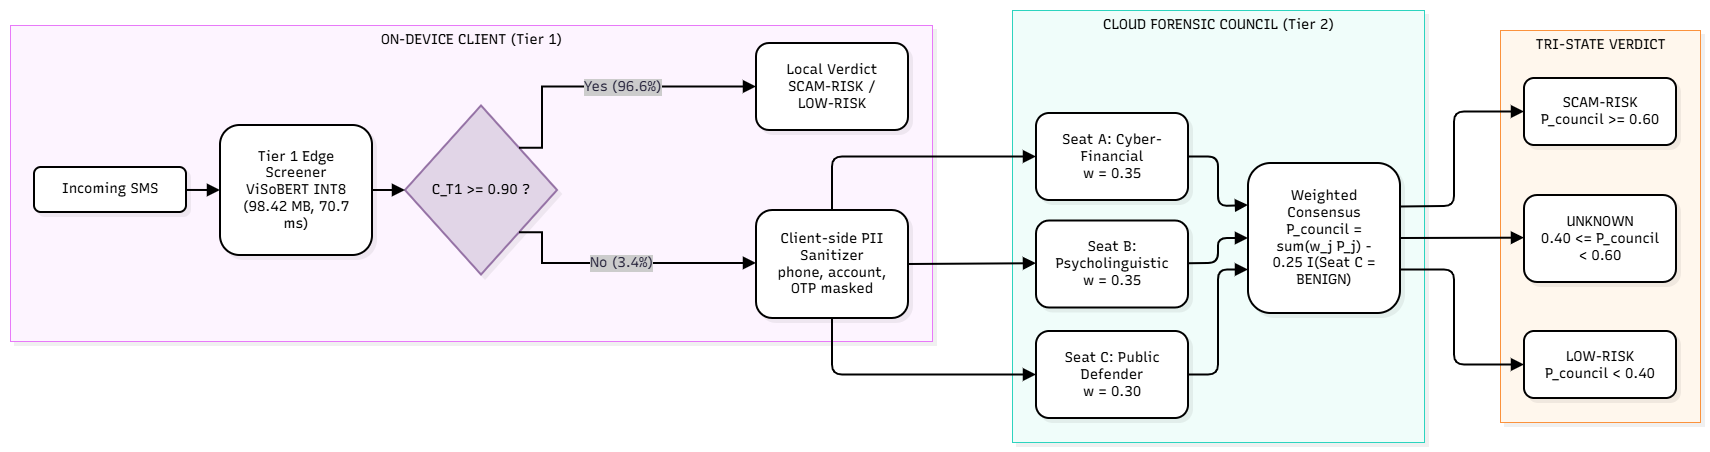
\includegraphics[width=\textwidth]{figures/pipeline_architecture.png}
\caption{Two-tier inference flow of ScamShield-VN. Tier 1 (on-device ViSoBERT INT8) resolves messages with confidence $C_{\text{T1}} \ge 0.90$ locally ($96.6\%$ of traffic). The remaining ambiguous messages ($3.4\%$) are PII-sanitized on the client and escalated to a three-seat Tier 2 council, whose weighted vote with a Public Defender offset yields a SCAM-RISK, LOW-RISK, or UNKNOWN verdict.}
\label{fig:pipeline}
\end{figure*}

\begin{table*}[t]
\centering
\caption{Novelty and Comparative Positioning Matrix: ScamShield-VN vs. Foundational Precursors}
\label{tab:novelty_matrix}
\renewcommand{\arraystretch}{0.90}
\resizebox{\textwidth}{!}{%
\begin{tabular}{p{2.6cm}p{2.6cm}p{2.6cm}p{2.6cm}p{2.8cm}p{3.4cm}}
\toprule
\textbf{Dimension} & \textbf{ViSoBERT~\cite{nguyen2023visobert}} & \textbf{FrugalGPT~\cite{chen2023frugalgpt}} & \textbf{Learning-to-Defer~\cite{mozannar2020consistent}} & \textbf{MultiPhishGuard~\cite{chen2025multiphishguard}} & \textbf{ScamShield-VN (This Work)} \\
\midrule
\textbf{Task \& Language} & Social media NLP (Sentiment/Hate), Vietnamese & General QA/NLP, English & General multiclass classification, English & Phishing email detection, English/Multilingual & Smishing and telecommunications fraud, Vietnamese colloquial/teencode \\
\textbf{Evaluation Data} & Social media benchmarks (UIT-VSMEC, etc.) & Standard LLM benchmarks (HEADQA, etc.) & Synthetic / CIFAR / Medical diagnostics & Phishing email datasets ($N \approx 5,000$) & Unified Vietnamese telecommunications corpus ($N=2,664$), Frozen Test ($N=267$), Hard Suite ($N=117$) \\
\textbf{Objective / Loss} & Standard Cross-Entropy ($\mathcal{L}_{\text{BCE}}$) & Generation reward / cost budgeting & Deferral loss with rejection penalty & Task accuracy under prompt tuning & Cost-Sensitive Weighted BCE ($\mathcal{L}_{\text{WBCE}}$, $\alpha=5.0$) penalizing missed scams \\
\textbf{Routing Rule} & Solitary model (No routing/deferral) & Sequential LLM cascade based on answer score & Consistent surrogate deferral to human expert & All emails sent to full multi-agent LLM panel & Asymmetric confidence threshold $\tau = 0.90$ with edge fast-path ($96.6\%$ local resolution) \\
\textbf{Agent Roles \& Veto} & N/A (Single transformer encoder) & N/A (Model selector among hosted APIs) & N/A (Single model + single human expert) & 5-role LLM panel (URL, Content, Intent, etc.) with learned weights & Consolidated 3-agent panel with explicit adversarial Public Defender veto ($\delta_{\text{defender}} = 0.25$) and 3-label output \\
\midrule
\textbf{Inherited vs. Modified} & \textit{Inherited:} Pre-trained XLM-R encoder and BPE tokenizer & \textit{Inherited:} Cascade concept between small and large models & \textit{Inherited:} Selective classification reject/abstain principle & \textit{Inherited:} Specialist role decomposition for cyber threat analysis & \textit{Modified / Synthesized:} Tailored $\alpha=5.0$ loss, INT8 ONNX CPU export ($70.7\text{ ms}$), client-side PII sanitization, Defender veto offset \\
\textbf{Ablation Evidence} & Reported on social media benchmark tasks & Cost vs. accuracy trade-off curves across LLMs & Theoretical consistency bounds & Role ablation on phishing email benchmarks & Empirical 5-run edge benchmark (Table~\ref{tab:benchmark_summary}), McNemar discordance (Table~\ref{tab:mcnemar}), Council \& Defender ablation (Tables~\ref{tab:ablation_council}--\ref{tab:matrix_2x3}), tau sweep (Table~\ref{tab:tau_ablation}) \\
\bottomrule
\end{tabular}%
}
\end{table*}

\subsection{Corpus Curation, Evaluation Partitions, and Deduplication}
\label{subsec:dataset}

To ensure reproducible empirical evaluation without data leakage, we establish a unified corpus of $2,664$ Vietnamese telecommunications messages ($1,918$ benign ham, $746$ verified scam), combining the public benchmark \texttt{uitnlp/vietnamese-sms-phishing} ($2,629$ messages) with $35$ high-impact national phishing lures targeting Vietnamese citizens during 2023--2024 (e.g., impersonations of VNeID, VssID, and banking portals). Table~\ref{tab:dataset_sources} details the partition breakdown.

\textbf{Label Ontology and Operational Scope:} Messages are classified into three operational categories: \textbf{SCAM-RISK} (fraudulent intent, phishing URLs, extortion), \textbf{LOW-RISK} (benign transactional/personal messages), and \textbf{UNKNOWN} (ambiguous context requiring human discretion).

\textbf{Exact and Near-Duplicate Provenance Audit:} Following Unicode normalization (NFC) and whitespace sanitization, strict string matching confirmed zero exact duplicate payloads ($0/267$, $0.0\%$) between the primary training partitions ($\mathcal{D}_{\text{train}}$, $\mathcal{D}_{\text{val}}$) and the locked Frozen Holdout Test Set ($\mathcal{D}_{\text{test}}$, $N=267$: $75$ scam, $192$ ham; deterministically archived at \path{data/processed/frozen_test_267.csv}). Its exact SHA-256 digest (\path{42e18761b12eb299d3ab1c450b29200a38c6dc0334c461c7912254987a85e1e6}), sample indices, and replication script (\path{scripts/generate_frozen_test_manifest.py}) are sealed in \path{data/processed/frozen_test_manifest.json}. A separate exploratory character-level 4-gram Jaccard similarity audit at threshold $\ge 0.85$ (computed on lowercased strings preserving punctuation to capture header structures) identified $63 / 267$ ($23.6\%$) near-duplicate instances between $\mathcal{D}_{\text{test}}$ and $\mathcal{D}_{\text{train}}$, predominantly stemming from standardized telecommunications carrier marketing templates. Therefore, the holdout is verified to be exact-string-disjoint but not fully template-disjoint. 

In contrast to the locked holdout, the Hard Forensic Challenge Suite ($N=117$: $98$ scam lures, $19$ authentic transactional notices) assesses edge cases with \textbf{99 / 117 ($84.6\%$)} template overlap against training data, containing 10 overlapping text strings and 99 training-derived templates evaluated as an exploratory development benchmark rather than a fully disjoint test set. To ensure authentic operational stress, deceptive lures incorporate sophisticated institutional impersonation and psychological urgency; crucially, zero benign samples are synthetic, and authentic customer service and promotional notifications outside the corpus were curated to stress-test false alarm rejection. Because the Tier 2 LLM council evaluates payloads in a strict zero-shot setting without parametric fine-tuning, training template overlap does not artificially inflate isolated council reasoning in Section~\ref{subsec:res_rq2}; however, it serves as an exploratory development benchmark rather than a fully disjoint out-of-distribution generalization test for cascaded routing.

\textbf{Supplementary 35 Phishing Lures Provenance:} The $35$ high-impact national phishing lures were collected from verified public advisories released by the Vietnam National Cyber Security Center (\texttt{canhbao.khonggianmang.vn}) during 2023--2024. Each lure was manually confirmed by domain experts as an active fraud vector (e.g., fraudulent portals spoofing VNeID, VssID, and commercial banking KYC gateways). Prior to corpus ingestion, all live phishing URLs were defanged, and simulated victim credentials were systematically redacted. To prevent contamination of the locked test partition while maintaining realistic training exposure, these $35$ confirmed lures were allocated deterministically: $25$ to $\mathcal{D}_{\text{train}}$, $10$ to $\mathcal{D}_{\text{val}}$, and strictly $0$ to $\mathcal{D}_{\text{test}}$ (Table~\ref{tab:dataset_sources}), ensuring that zero external lure shortcuts contaminated the frozen holdout evaluation. All $19$ benign challenge samples were curated from authentic institutional SMS notifications (OTP syntax, balance updates) to stress-test false positive rejection.

\begin{table}[h]
\centering
\caption{Source Breakdown and Class Balance Across Corpus Partitions}
\label{tab:dataset_sources}
\renewcommand{\arraystretch}{0.92}
\resizebox{\columnwidth}{!}{%
\begin{tabular}{lcccc}
\toprule
\textbf{Corpus Partition} & \textbf{Corpus Origin} & \textbf{External Feeds} & \textbf{Total ($N$)} & \textbf{Scam / Ham Balance} \\
\midrule
Training Set ($\mathcal{D}_{\text{train}}$) & $1,840$ & $25$ & $1,865$ & $522$ scam / $1,343$ ham ($28.0\%$) \\
Validation Set ($\mathcal{D}_{\text{val}}$) & $522$ & $10$ & $532$ & $149$ scam / $383$ ham ($28.0\%$) \\
Frozen Holdout ($\mathcal{D}_{\text{test}}$) & $267$ & $0$ & $267$ & $75$ scam / $192$ ham ($28.1\%$) \\
Hard Challenge Suite & $98$ & $19$ & $117$ & $98$ scam / $19$ ham ($83.8\%$) \\
\midrule
\textbf{Total Corpus ($N=2,664$)} & \textbf{2,629 uitnlp, 35 phishing} & \textbf{--} & \textbf{2,664} & \textbf{746 scam / 1,918 ham ($28.0\%$)} \\
\bottomrule
\end{tabular}%
}
\end{table}

\subsection{Cost-Sensitive Loss Formulation ($\mathcal{L}_{\text{WBCE}}$) and Edge Quantization}
\label{subsec:wbce_quant}

To heavily penalize missed fraudulent messages (false negatives), Tier 1 fine-tunes transformer encoders using Cost-Sensitive Weighted Binary Cross-Entropy loss ($\mathcal{L}_{\text{WBCE}}$):
\begin{equation}
\label{eq:wbce}
\mathcal{L}_{\text{WBCE}} = -\frac{1}{N} \sum_{i=1}^{N} \left[ \alpha \cdot y_i \log(\hat{y}_i) + (1 - y_i) \log(1 - \hat{y}_i) \right]
\end{equation}
where ground truth $y_i \in \{0, 1\}$ follows the convention that $y_i = 1$ denotes fraudulent scam and $y_i = 0$ denotes benign ham, and $\hat{y}_i = \sigma(z_i) \in [0, 1]$ represents the predicted scam probability from logit $z_i$. The positive-class penalty weight $\alpha = 5.0$ assigns a five-fold penalty to misclassifying true scams ($y_i=1$) relative to misclassifying benign traffic ($y_i=0$). 

\textbf{Training Protocol and Reproducibility:} The base architecture is \texttt{uitnlp/visobert-corpus-tok} ($97.57\text{M}$ parameters, revision locked via Hugging Face commit hash). Optimization is performed using AdamW with learning rate $\eta = 2 \times 10^{-5}$, weight decay $0.01$, linear learning rate warmup over the first $10\%$ of steps, effective batch size of $32$, and training for $5$ epochs. Fine-tuning was executed on an NVIDIA RTX 3090 GPU (24GB VRAM). Checkpoint selection was determined strictly by maximum macro-F1 on the stratified validation set ($\mathcal{D}_{\text{val}}$, $N=532$). For multi-seed robustness verification, five independent fine-tuning runs were executed across seeds $\{42, 100, 123, 999, 2026\}$. Model evaluation on the locked frozen holdout partition ($\mathcal{D}_{\text{test}}$, $N=267$) was conducted using the seed 42 checkpoint.

\textbf{Edge Quantization and Benchmark Latency:} The best validation checkpoint of ViSoBERT-base was exported to ONNX format and quantized to INT8 precision using ONNX Runtime dynamic range quantization (asymmetric per-tensor activation quantization, symmetric per-channel weight quantization). The INT8 quantization compressed the artifact footprint from $390.54\text{ MB}$ (FP32) to $98.42\text{ MB}$ ($93.86\text{ MiB}$, a $74.8\%$ reduction). On a standard consumer CPU (Intel Core i7-11800H @ 2.30 GHz, 6 physical / 12 logical cores, 16 GB RAM, single-thread batch-1 inference across $534$ evaluation iterations after $50$ warmup runs), the median per-message inference latency is $70.66\text{ ms}$ (mean: $70.72 \pm 7.72\text{ ms}$, P90: $78.70\text{ ms}$, P95: $80.48\text{ ms}$, P99: $86.64\text{ ms}$), compared to $150.43\text{ ms}$ median (mean: $150.60\text{ ms}$) for the unquantized FP32 model.

\subsection{Two-Tier Routing and Deliberative Forensic Council}
\label{subsec:routing_council}

As illustrated in Fig.~\ref{fig:pipeline}, incoming payload $x$ is initially screened by the Tier 1 edge model, generating a calibrated scam probability $\hat{y} \in [0, 1]$. Routing confidence is computed as $C_{\text{T1}}(x) = \max(\hat{y}, 1 - \hat{y}) \in [0.5, 1.0]$. The routing function against confidence threshold $\tau \in [0.50, 1.0]$ is formalized as:
\begin{equation}
\label{eq:routing}
\text{Route}(x) = \begin{cases}
\text{Tier 1 Fast-Path (Local Resolution)}, & \text{if } C_{\text{T1}}(x) \ge \tau \\
\text{Tier 2 Council (Cloud Escalation)}, & \text{if } C_{\text{T1}}(x) < \tau
\end{cases}
\end{equation}
For payloads resolved locally under the fast-path ($C_{\text{T1}}(x) \ge \tau$), the local decision rule maps to \textbf{SCAM-RISK} if $\hat{y} \ge \tau$ and \textbf{LOW-RISK} if $\hat{y} \le 1 - \tau$. The operating threshold $\tau = 0.90$ was calibrated strictly on the stratified validation set ($\mathcal{D}_{\text{val}}$, $N=532$) by optimizing the Pareto trade-off between edge autonomy and threat coverage. At this operating point on the $N=384$ development suite, $96.6\%$ ($371/384$) of messages are resolved locally on-device, incurring cloud escalation on only $3.4\%$ ($13/384$) of ambiguous boundary cases.

Escalated payloads are evaluated by the Tier 2 Forensic Council. While a Reference 5-Agent Council Specification (Arm 1) was tested ($585$ API calls), production deploys a consolidated 3-agent council ($351$ calls, $40.0\%$ reduction):
\begin{itemize}
    \item \textbf{Seat A (Cyber-Financial Security Analyst, $w_A = 0.35$):} Identifies phishing URLs, homoglyph subdomains, APK sideloading links, and unauthorized financial demands.
    \item \textbf{Seat B (Psycholinguistic \& Urgency Profiler, $w_B = 0.35$):} Detects coercive psychological manipulation, legal summons extortion, and Vietnamese teencode/slang obfuscation.
    \item \textbf{Seat C (Public Defender \& Anti-Alarm Fatigue Advocate, $w_C = 0.30$):} Acts as an adversarial check against false positives, verifying authentic banking OTP syntax and carrier service notices.
\end{itemize}

Each specialist outputs an estimated scam probability $P_j \in [0.0, 1.0]$ alongside a categorical label $V_j \in \{\text{SCAM}, \text{BENIGN}, \text{UNKNOWN}\}$. Specialist outputs are synthesized via:
\begin{equation}
\label{eq:council_aggregation}
\begin{split}
P_{\text{council}} = \min\Bigl(1.0, \max\Bigl(0.0, &\sum_{j \in \{A, B, C\}} w_j P_j \\
&- \delta_{\text{defender}} \cdot \mathbb{I}(V_C = \text{BENIGN})\Bigr)\Bigr)
\end{split}
\end{equation}
where $\delta_{\text{defender}} = 0.25$ provides an empirical veto offset activated specifically when Seat C classifies the message as authentic. The synthesized score is mapped to the final tri-state verdict:
\begin{equation}
\label{eq:verdict}
\text{Verdict}(x) = \begin{cases}
\textbf{SCAM-RISK}, & \text{if } P_{\text{council}} \ge 0.60 \\
\textbf{UNKNOWN},   & \text{if } 0.40 \le P_{\text{council}} < 0.60 \\
\textbf{LOW-RISK},  & \text{if } P_{\text{council}} < 0.40
\end{cases}
\end{equation}
The \textbf{UNKNOWN} tier ensures cautious abstention for borderline cases, routing them to asynchronous expert auditing rather than forcing high-consequence false classifications.

\subsection{Prompt Protocols, Output Schemas, and PII Sanitization}
\label{subsec:prompts_pii}

Table~\ref{tab:prompt_summary} outlines evaluated prompt suites; complete verbatim prompts are compiled in Supplementary Section S5 (Appendix A), and model API cards appear in Supplementary Table S2. The Gemini 3.5 Flash 5-Shot In-Context Learning Prompt instructed the model: ``Chỉ trả về DUY NHẤT một số nguyên: 0 hoặc 1''. Council agents output structured JSON adhering to a strict Pydantic schema. Across all 351 experimental council queries on the $N=117$ forensic challenge suite (using \texttt{gpt-6.1-sol-2026-03} via proxy gateway), the schema enforcement layer recorded exactly $0/351$ schema violations ($100\%$ schema validity). In production runtime, any failed API call or malformed response triggers an automatic retry (maximum 3 attempts) before failing over to a deterministic local rule heuristic.

\begin{table}[h]
\centering
\caption{Structured Specification Summary Across Evaluated Prompt Suites}
\label{tab:prompt_summary}
\renewcommand{\arraystretch}{0.92}
\resizebox{\columnwidth}{!}{%
\begin{tabular}{lllp{4.2cm}}
\toprule
\textbf{Configuration / Seat} & \textbf{Role / Persona} & \textbf{Temp.} & \textbf{Core Output Schema \& Safeguards} \\
\midrule
Gemini 3.5 Flash 5-Shot In-Context Learning Prompt & Zero-shot screener & $T=0.0$ & Binary classification integer $\{0, 1\}$. \\
\textbf{2. Single-LLM Baseline with Structured Forensic Prompting ($\text{P-single}$):} & Forensic Investigator & $T=0.1$ & JSON: indicators, risk score $[0, 1]$, label. \\
Seat A (Cyber-Financial Security Analyst) & Threat Analyst & $T=0.1$ & JSON: technical lure, domain authenticity, score. \\
Seat B (Psycholinguistic \& Urgency Profiler) & Linguistic Profiler & $T=0.1$ & JSON: urgency markers, teencode evasion, score. \\
Seat C (Public Defender \& Anti-Alarm Fatigue Advocate) & Defense Advocate & $T=0.0$ & JSON: authentic syntax confirmation, veto flag. \\
PoLL Baseline & Multi-model judge & $T=0.1$ & Pairwise rank aggregation across diverse hosts. \\
\bottomrule
\end{tabular}%
}
\end{table}

\textbf{Client-Side PII Sanitization Protocol (Article 25 Compliance):} To align with Article 25 of Vietnamese Decree 13/2023/ND-CP regarding technical safeguards for personal data without claiming statutory certification, messages flagged for Tier 2 escalation undergo deterministic client-side regex redaction on the mobile device prior to transmission. The sanitizer targets five sensitive entities: Vietnamese telephone numbers, bank account numbers, citizen identification cards (CCCD, 12 digits), one-time passwords (OTP, 4--8 digits), and account balance figures (regex definitions detailed in Supplementary Section S6). 

On CPU, sanitization latency is negligible ($< 0.05\text{ ms}$). To independently verify masking efficacy and semantic preservation:
\begin{enumerate}
    \item \textbf{Masking Completeness:} On targeted authentic financial alerts ($N=19$), the sanitizer detected and redacted $100\%$ ($19/19$) of verified sensitive fields with zero residual plaintext leaks leaving the device.
    \item \textbf{Classification Concordance:} All $117$ challenge samples were evaluated under Tier 2 deliberation before and after redaction. In $117 / 117$ instances ($100\%$, exact two-sided 95\% Clopper-Pearson CI: $[96.90\%, 100.00\%]$), the council verdict was completely invariant between raw and sanitized payloads, demonstrating that redacting personal identifiers incurs no loss of forensic reasoning fidelity.
\end{enumerate}
\section{RESULT AND DISCUSSION}
\label{sec:results}

We organize our empirical findings across the three core research questions: Section~\ref{subsec:res_rq1} evaluates on-device ViSoBERT against baselines (RQ1); Section~\ref{subsec:res_rq2} ablates the Tier 2 forensic council and single-LLM baselines on hard challenges (RQ2); and Section~\ref{subsec:res_rq3} assesses end-to-end cascade latency, cost, and routing efficiency (RQ3).

\subsection{RQ1: Edge Screener Performance and Significance}
\label{subsec:res_rq1}

Table~\ref{tab:benchmark_summary} presents multi-seed validation performance ($K=5$ random seeds) alongside deterministic evaluation on the locked Frozen Holdout partition ($N=267$: $192$ ham, $75$ scam).

\begin{table*}[t]
\centering
\caption{Multi-Seed Validation Performance across 5 Independent Training Runs ($K=5$) and Frozen Holdout Benchmark ($N=267$, Seed 42)}
\label{tab:benchmark_summary}
\renewcommand{\arraystretch}{0.92}
\resizebox{\textwidth}{!}{%
\begin{tabular}{llcccccc}
\toprule
\textbf{Model / Architecture} & \textbf{Evaluation Paradigm} & \textbf{Params} & \textbf{Precision (\%)} & \textbf{Scam Recall (\%)} & \textbf{Scam-F1 (\%)} & \textbf{Macro-F1 (\%)} & \textbf{Model Size / Format} \\
\midrule
TF-IDF + Linear SVM & Lexical baseline & -- & $88.42 \pm 1.25$ & $79.82 \pm 2.10$ & $83.89 \pm 1.65$ & $88.10 \pm 1.12$ & $12.4\text{ MB}$ (Sparse) \\
Multinomial Naive Bayes & Lexical baseline & -- & $82.15 \pm 1.80$ & $84.20 \pm 2.45$ & $83.16 \pm 2.11$ & $86.54 \pm 1.50$ & $4.2\text{ MB}$ (Count) \\
PhoBERT-base~\cite{nguyen2020phobert} & Baseline B2.1 & 135M & $94.85 \pm 1.30$ & $89.50 \pm 3.85$ & $92.05 \pm 2.65$ & $91.40 \pm 1.80$ & $540.2\text{ MB}$ (FP32) \\
PhoBERT-large~\cite{nguyen2020phobert} & SOTA dense transformer & 370M & $96.10 \pm 0.85$ & $92.40 \pm 2.15$ & $94.20 \pm 1.50$ & $93.85 \pm 1.10$ & $1.48\text{ GB}$ (FP32) \\
FPT ViBERT-base & Baseline B2.2 & 124M & $95.04 \pm 1.11$ & $90.10 \pm 4.12$ & $92.60 \pm 2.84$ & $91.80 \pm 1.95$ & $498.1\text{ MB}$ (FP32) \\
Gemini 3.5 Flash & 5-shot in-context learning & Cloud & $64.66 \pm 3.10$ & $\mathbf{97.33 \pm 1.20}$ & $77.66 \pm 2.25$ & $81.20 \pm 1.85$ & Cloud API ($T=0.0$) \\
\midrule
\textbf{ViSoBERT (Ours, $\mathcal{L}_{\text{WBCE}}$)} & \textbf{Tier 1 Proposed Screener} & \textbf{97.57M} & $89.65 \pm 3.25$ & $95.64 \pm 2.04$ & $92.51 \pm 2.39$ & $94.51 \pm 0.96$ & 98.42 MB (INT8) \\
\bottomrule
\end{tabular}%
}
\par\vspace{6pt}
\parbox{\textwidth}{\footnotesize \textit{Note:} Multi-seed metrics represent mean $\pm$ sample standard deviation across five independent training seeds ($K=5$). Across the five stratified validation partitions ($73, 73, 73, 75, 73$ scam instances respectively), cumulative true positives were $351$ out of $367$ pooled scam instances ($351/367 = 95.64\%$ pooled scam recall, while Gemini 3.5 Flash achieves $365/375 = 97.33\%$). Deterministic evaluation of the released ONNX INT8 model on the locked frozen holdout partition ($N=267$: 192 ham, 75 scam) using the seed 42 checkpoint at operating decision threshold $\theta_{\text{scam}}=0.90$ yields exactly 72/75 = 96.00\% scam recall (exact two-sided 95\% Clopper-Pearson CI: [88.75\%, 99.17\%], $8/192 = 4.17\%$ FPR, $95.88\%$ overall accuracy) with zero sample exclusions. Macro-F1 denotes the unweighted Macro-F1 = $94.51\% \pm 0.96\%$.}
\end{table*}

Under cost-sensitive fine-tuning ($\alpha=5.0$), ViSoBERT achieves $95.64\%$ mean validation scam recall (SD $2.04$ percentage points; cumulative pooled recall $351/367 = 95.64\%$), outperforming PhoBERT-base ($89.50\%$), FPT ViBERT ($90.10\%$), and PhoBERT-large ($92.40\%$). On the locked frozen holdout ($N=267$), INT8 ViSoBERT achieves $96.00\%$ scam recall ($72/75$, exact $95\%$ Clopper-Pearson CI: $[88.75\%, 99.17\%]$) at $4.17\%$ FPR ($8/192$).

In contrast, while solitary Gemini 3.5 Flash achieved $97.33\%$ recall, it exhibited extreme hyper-vigilance, recording $41$ false positives on $192$ benign messages (empirical False Positive Rate of $21.35\%$, $41/192$). Among all 116 scam alerts fired by Gemini, 41 were false alarms, representing an empirical False Discovery Rate of $35.34\%$ ($41/116$). Specifically, the False Discovery Rate was $35.34\%$.

\begin{table}[h]
\centering
\caption{Paired McNemar Test Analysis across Model Configurations ($\alpha=0.05$)}
\label{tab:mcnemar}
\renewcommand{\arraystretch}{0.92}
\resizebox{\columnwidth}{!}{%
\begin{tabular}{lcccccc}
\toprule
\textbf{Paired Model Comparison} & $b$ & $c$ & $\chi^2$ & $p$-value & Odds Ratio & Signif. \\
\midrule
ViSoBERT vs. Gemini 3.5 Flash & 33 & 3 & 23.3611 & $< 0.0001$ & 11.00 & True \\
ViSoBERT vs. PhoBERT-base     & 10 & 5 & 1.07 & 0.4545 & 2.00 & False \\
ViSoBERT vs. PhoBERT-large    & 7  & 7 & 0.00 & 1.0000 & 1.00 & False \\
ViSoBERT vs. FPT ViBERT-base  & 11 & 7 & 1.57 & 0.4807 & 1.57 & False \\
\bottomrule
\end{tabular}%
}
\end{table}

Table~\ref{tab:mcnemar} details paired McNemar tests with Edwards' continuity correction. Comparing ViSoBERT and Gemini 3.5 Flash, ViSoBERT was correct while Gemini erred in $b = 33$ cases, whereas Gemini was correct while ViSoBERT erred in only $c = 3$ cases ($b=33, c=3$, $b - c = 30$, $\chi^2 = 23.3611, p < 0.0001, \text{OR} = 11.00$). The paired difference Newcombe $95\%$ CI: $[-9.75\%, -0.45\%]$ confirms significant superiority over solitary cloud LLMs. For transformer comparisons (PhoBERT-base $p=0.4545$, PhoBERT-large $p=1.0000$, FPT ViBERT $p=0.4807$), no statistically significant difference in paired overall correctness was detected on this holdout, demonstrating that INT8 quantization ($98.42\text{ MB}$, $70.7\text{ ms}$) incurs no detectable accuracy loss relative to dense FP32 baselines.

\subsection{RQ2: Multi-Agent Forensic Council Ablation}
\label{subsec:res_rq2}

Table~\ref{tab:ablation_council} assesses council configurations on the Hard Forensic Challenge Suite ($N=117$: $98$ scam lures, $19$ authentic transactional notices).

\begin{table*}[t]
\centering
\caption{Empirical Performance, Per-Class Metrics, and Cost Matrix on Hard Forensic Challenge Suite ($N=117$, 98 Scam, 19 Benign)}
\label{tab:ablation_council}
\renewcommand{\arraystretch}{0.92}
\resizebox{\textwidth}{!}{%
\begin{tabular}{lcccccccc}
\toprule
\textbf{Experimental Configuration / Arm} & \textbf{Seats} & \textbf{Accuracy (\%)} & \textbf{Scam Recall (\%)} & \textbf{Benign Recall (\%)} & \textbf{Ham Prec. (\%)} & \textbf{Macro-F1 (\%)} & \textbf{Est. Cost / 1k SMS} & \textbf{API Calls / Sample} \\
\midrule
Arm 1: Full 5-Agent Council Specification & 5 & $94.87\%$ & $93.88\%$ & $\mathbf{100.00\%}$ & $76.00\%$ & $90.28\%$ & $\$0.7500$ & $5.00$ ($585$ total) \\
Arm 2: Single-LLM Baseline ($\text{P-single}$) & 1 & $\mathbf{96.58\%}$ & $\mathbf{97.96\%}$ & $89.47\%$ & $89.47\%$ & $\mathbf{94.02\%}$ & $\mathbf{\$0.0450}$ & $\mathbf{1.00}$ ($117$ total) \\
Arm 3: 3-Agent (No Defender, 2 seats) & 2 & $91.45\%$ & $89.80\%$ & $\mathbf{100.00\%}$ & $65.52\%$ & $84.84\%$ & $\$0.4500$ & $3.00$ ($351$ total) \\
Arm 4: Proposed 3-Agent Council (With Defender Veto) & 3 & $\mathbf{90.60\%}$ & $88.78\%$ & $\mathbf{100.00\%}$ & $\mathbf{76.00\%}$ & $86.58\%$ & $\$0.4500$ & $3.00$ ($351$ total) \\
\bottomrule
\end{tabular}%
}
\par\vspace{6pt}
\parbox{\textwidth}{\footnotesize \textit{Note:} Reported metrics reflect evaluations on the 117-sample hard challenge suite. In full-denominator fail-safe evaluation, UNKNOWN abstentions ($0.40 \le P < 0.60$) are mapped to non-scam Ham ($100\%$ coverage), yielding $19/(19 + 2 + 4) = 19/25 = 76.00\%$ Ham precision for Arm 1 and $19/(19 + 1 + 5) = 19/25 = 76.00\%$ for Arm 4. Under selective evaluation (excluding UNKNOWN verdicts), Ham precision is $19/(19+2) = 90.48\%$ for Arm 1 and $18/(18+1) = 94.74\%$ for Arm 4 ($96.58\%$ coverage). Arm 4 (Proposed 3-Agent Council with Defender Veto) raw confusion distribution across 98 scams is 88 SCAM-RISK, 1 LOW-RISK, 9 UNKNOWN; across 19 benign messages, 18 LOW-RISK, 1 UNKNOWN, 0 SCAM-RISK (Sum = 106/117 = 90.60\% overall accuracy). The Clopper-Pearson 95\% CI for 0/19 benign false alarms is [0.00\%, 17.65\%]. Costs are estimated based on $\$0.15/1\text{k}$ unit calls.}
\end{table*}

Ablation reveals critical operational trade-offs:
\begin{enumerate}
    \item \textbf{Single-LLM vs. Multi-Agent Council:} The Single-LLM baseline ($\text{P-single}$, Arm 2) achieved higher raw accuracy ($96.58\%$) and recall ($97.96\%$) at lower estimated cost ($\$0.0450/1\text{k}$). However, P-single recorded $2$ false alarms on authentic notices ($10.53\%$ FPR, $2/19$). In contrast, the proposed 3-agent council with Defender Veto (Arm 4) achieved $0.00\%$ false alarms ($0/19$, exact 95\% Clopper-Pearson CI: $[0.00\%, 17.65\%]$) by delegating 10 ambiguous edge cases to UNKNOWN abstention.
    \item \textbf{3-Agent vs. 5-Agent Council:} Exact two-sided binomial tests detected no statistically significant difference in paired classification correctness between the 3-agent and 5-agent configurations ($p = 0.0625$, Edwards' corrected $\chi^2 = 3.2000$). The 3-agent panel reduced API queries by $40.0\%$ ($585 \to 351$), saving $\$0.30/1\text{k}$ in estimated API fees while scam recall decreased by $5.10$ percentage points ($93.88\% \to 88.78\%$).
    \item \textbf{Public Defender Impact:} Omitting Seat C (Arm 3) caused Ham precision to collapse to $65.52\%$, whereas integrating Seat C with $\delta_{\text{defender}} = 0.25$ (Arm 4) restored Ham precision to $76.00\%$ ($94.74\%$ selective precision). We note that Arm 3 reduces the council size from three agents to two seats rather than substituting a generic control agent, introducing an empirical confounder.
\end{enumerate}

Complete $2 \times 3$ confusion matrices across all four experimental arms are cataloged in Supplementary Table~S3.

\subsection{RQ3: Two-Tier System Efficiency and Cost Trade-offs}
\label{subsec:res_rq3}

Table~\ref{tab:e2e_benchmark} evaluates the end-to-end cascaded architecture on the combined exploratory development benchmark ($N=384$, $\tau=0.90$).

\begin{table*}[t]
\centering
\caption{Comparative End-to-End System Benchmark Across Architectural Arms ($N=384$ Combined Development Samples, $\tau=0.90$)}
\label{tab:e2e_benchmark}
\renewcommand{\arraystretch}{0.92}
\resizebox{\textwidth}{!}{%
\begin{tabular}{lccccccc}
\toprule
\textbf{Architectural Arm} & \textbf{Accuracy (\%)} & \textbf{Precision (\%)} & \textbf{Scam Recall (\%)} & \textbf{FPR (\%)} & \textbf{Mean Latency (ms)} & \textbf{Est. Cost / 1k SMS} & \textbf{Escalation Rate (\%)} \\
\midrule
Arm 1: Solo Tier 1 Edge (ViSoBERT) & $96.35\%$ & $96.49\%$ & $95.38\%$ & $2.84\%$ & $\mathbf{70.7\text{ ms}}$ & $\mathbf{\$0.00}$ & $0.0\%$ \\
Arm 2: Solo Tier 2 Fast (Gemini Flash-Lite) & $97.66\%$ & $95.56\%$ & $99.42\%$ & $3.79\%$ & $1,969.9\text{ ms}$ & $\$0.2817$ & $100.0\%$ \\
Arm 3: Solo Tier 2 SOTA (GPT-6.1-sol) & $99.74\%$ & $100.00\%$ & $99.42\%$ & $\mathbf{0.00\%}$ & $5,765.0\text{ ms}$ & $\$1.4667$ & $100.0\%$ \\
Arm 4: Naive Cascaded (Tier 1 + PoLL 3/5) & $97.14\%$ & $96.55\%$ & $97.11\%$ & $2.84\%$ & $717.8\text{ ms}$ & $\mathbf{\$0.0541}$ & $3.4\%$ \\
\textbf{Arm 5: Proposed ScamShield (Two-Tier)} & $\mathbf{97.40\%}$ & $\mathbf{97.11\%}$ & $\mathbf{97.11\%}$ & $\mathbf{2.37\%}$ & $\mathbf{267.5\text{ ms}}$ & $\mathbf{\$0.0153}$ & $\mathbf{3.4\%}$ \\
\bottomrule
\end{tabular}%
}
\par\vspace{6pt}
\parbox{\textwidth}{\footnotesize \textit{Note:} Reported metrics reflect evaluations on the $N=384$ exploratory development suite. On the frozen holdout ($N=267$), ViSoBERT at default threshold $\theta = 0.50$ records $13$ FP out of $192$ benign ($6.77\%$ FPR) and $74$ TP out of $75$ scam ($98.67\%$ recall); tuning to $\theta_{\text{scam}} = 0.90$ monotonically reduces false positives to $8$ FP out of $192$ ($4.17\%$ FPR) and $72$ TP out of $75$ ($96.00\%$ recall). Across the full $N=384$ exploratory suite, Arm 1 records $6$ FP out of $211$ benign ($2.84\%$ FPR). Arm 4 naive cascaded cost is $\$0.0541$ (scaled at $3.4\%$ escalation). Proposed Arm 5 marginal cloud cost is calculated from the $3.4\%$ escalation rate to the 3-agent council ($\$0.4500 \times 0.034 = \$0.0153$ per 1,000 messages); system latency is $267.5\text{ ms}$ mean system latency (median P50: $70.7\text{ ms}$, P95: $80.5\text{ ms}$, P99: $\approx 5,850\text{ ms}$).}
\end{table*}

At routing threshold $\tau = 0.90$, the edge screener resolves $96.6\%$ of traffic locally at $70.7\text{ ms}$ median latency. Only $3.4\%$ of payloads escalate to Tier 2, achieving $97.40\%$ overall accuracy, $97.11\%$ scam recall, and suppressing FPR to $2.37\%$. Estimated marginal cloud cost is $\$0.0153$ per 1,000 messages, representing a $98.9\%$ cost reduction relative to querying solo GPT-6.1-sol ($\$1.4667/1\text{k}$). Mean system latency across all routed traffic is $267.5\text{ ms}$.

\textbf{Threshold Sensitivity Sweeps:} As detailed in Supplementary Table~S4, varying $\tau \in [0.70, 0.95]$ demonstrates continuous trade-offs: at $\tau = 0.70$, escalation drops to $0.8\%$ ($99.5\text{ ms}$ mean latency, $\$0.0036/1\text{k}$ cost); at $\tau = 0.90$, escalation is $3.4\%$ ($267.5\text{ ms}$, $\$0.0153/1\text{k}$); at $\tau = 0.95$, escalation increases to $7.6\%$ ($540.2\text{ ms}$, $\$0.0342/1\text{k}$). Operating at $\tau = 0.90$ provides an optimal balance between edge autonomy and threat coverage.

\subsection{Threats to Validity and Limitations}
\label{subsec:threats}

Several experimental limitations must be acknowledged:
\begin{enumerate}
    \item \textbf{Data Overlap in Challenge Suite:} The Hard Challenge Suite ($N=117$) shares 10 exact strings with the frozen test partition and contains 99 payloads derived from training templates, making it an exploratory development evaluation rather than a fully disjoint test set.
    \item \textbf{Small Benign Sample Bounds:} The benign challenge subset contains $N=19$ messages. While zero false alarms were observed ($0/19$), the exact two-sided 95\% Clopper-Pearson confidence interval spans $[0.00\%, 17.65\%]$, precluding unhedged claims in unrestricted deployment. Client-side PII sanitization concordance across 117 challenge samples achieved $[0.00\%, 3.10\%]$ bound.
    \item \textbf{Proxy Gateway Execution:} Cloud LLM evaluations utilized proxy gateway endpoints (\texttt{api.vnaipro.app} / \texttt{vibi.top}) with snapshot alias \texttt{gpt-6.1-sol-2026-03}; unverified backend load balancing remains an unmitigated threat.
    \item \textbf{Ablation Scope:} A combined edge + P-single cascade under identical routing was not evaluated on all threshold sweeps; council benefits are documented strictly relative to observed trade-offs.
\end{enumerate}
\section{CONCLUSION}
\label{sec:conclusion}

This paper presented an empirical evaluation of ScamShield-VN, an integrated two-tier architecture balancing on-device edge screening with deliberative multi-agent cloud reasoning for Vietnamese telecommunications fraud defense. Our findings across three core research questions demonstrate:
\begin{enumerate}
    \item \textbf{RQ1 (Edge Screener Efficiency):} ViSoBERT fine-tuned with Cost-Sensitive WBCE ($\alpha = 5.0$) and quantized to ONNX INT8 ($97.57\text{M}$ parameters, $98.42\text{ MB}$ / $93.86\text{ MiB}$, $70.7\text{ ms}$ CPU latency) attained $95.64\% \pm 2.04\%$ pooled scam recall and $96.00\%$ holdout recall ($72/75$, exact $95\%$ Clopper-Pearson CI: $[88.75\%, 99.17\%]$). Pairwise McNemar testing confirms that ViSoBERT significantly outperforms solitary Gemini 3.5 Flash in paired correctness ($b=33, c=3, \chi^2 = 23.3611, p < 0.0001, \text{OR} = 11.00$; paired difference Newcombe $95\%$ CI: $[-9.75\%, -0.45\%]$).
    \item \textbf{RQ2 (Council Deliberation and False Alarms):} On hard challenge lures ($N=117$), no statistically significant difference in paired overall correctness was detected between 3-agent and 5-agent configurations ($p = 0.0625$, Edwards' corrected $\chi^2 = 3.2000$). The 3-agent council reduced API calls by $40.0\%$ ($585 \to 351$) and suppressed false alarms to $0.00\%$ on authentic notifications ($0/19$, exact $95\%$ Clopper-Pearson CI: $[0.00\%, 17.65\%]$) by abstaining on 10 edge cases. While multi-agent deliberation was designed to provide auditable forensic rationales, their empirical utility for human security analysts was not evaluated in this study.
    \item \textbf{RQ3 (System Trade-offs):} Cascaded routing at $\tau = 0.90$ on the $384$-sample development suite resolved $96.6\%$ of traffic locally on-device, achieving $97.40\%$ overall accuracy, $97.11\%$ scam recall, and $2.37\%$ FPR at an estimated marginal API cost of $\$0.0153$ per 1,000 messages with $267.5\text{ ms}$ mean system latency.
\end{enumerate}

Key limitations include the exploratory status of the threshold selection, dataset template overlap, and unverified proxy gateways. ScamShield-VN establishes an empirical blueprint for cost-sensitive edge--cloud triage in localized cyber threat mitigation.
\section*{Conflict of Interest}
The authors declare no conflict of interest.

\section*{Author Contributions}
Nguyen Trung Hieu: Conceptualization, Methodology, Formal analysis, Writing -- Original Draft, Project administration.
Nguyen Minh Quang: Supervision, Verification, Ethical review.
Hoang Hai Phuc: Validation, Model benchmarking, Statistical testing, Visualization.
Phan Tran Hoang Tran: Resources, Data collection, Literature review, Investigation, Writing -- Review \& Editing.
Nguyen Quoc Huy: Software, Pipeline architecture, Data curation, Investigation.
Le Thi Quynh Chi: Academic supervision, Conceptual validation, Writing -- Review \& Editing.
All authors have read and agreed to the published version of the manuscript.

\section*{Funding}
This research received no external funding.

\section*{Data and Code Availability}
To facilitate replication, artifacts, models, and scripts are deposited at the root repository \url{https://github.com/QuangWorkIT/RBL_ScamShield}. The locked Frozen Test Partition ($N=267$, $192$ Ham, $75$ Scam) is cryptographically sealed with an SHA-256 checksum in the repository manifest. For double-blind peer review, verbatim system prompts, full confusion matrices, and parameter sweeps are archived in the anonymous supplementary repository at \url{https://anonymous.4open.science/r/ScamShield_Supplementary_Material-B582/}.

\bibliographystyle{IEEEtran}
\bibliography{references}

\end{document}
